% =====================================================================
% Fundamentos de Sistemas Electrónicos Analógicos — Generador PWM TL494
% Compilar: pdflatex clase_4_tl494_pwm.tex  (2 pasadas)
% =====================================================================
\documentclass[aspectratio=169]{beamer}

\usepackage[utf8]{inputenc}
\usepackage[T1]{fontenc}
\usepackage{lmodern}
\usepackage[spanish,es-tabla]{babel}
\usepackage{amsmath,amssymb}
\usepackage{siunitx}
\usepackage{booktabs}
\usepackage{microtype}
\usepackage{circuitikz}

\definecolor{navy}{RGB}{23,54,93}
\definecolor{navysoft}{RGB}{72,101,140}
\definecolor{gold}{RGB}{179,142,62}
\definecolor{ink}{RGB}{44,51,58}
\definecolor{soft}{RGB}{244,241,234}
\definecolor{ox}{RGB}{214,120,40}

\usetheme{default}
\setbeamertemplate{navigation symbols}{}
\setbeamertemplate{footline}[frame number]
\setbeamercolor{structure}{fg=navy}
\setbeamercolor{frametitle}{fg=white,bg=navy}
\setbeamercolor{title}{fg=navy}
\setbeamercolor{subtitle}{fg=navysoft}
\setbeamercolor{itemize item}{fg=gold}
\setbeamercolor{itemize subitem}{fg=gold}
\setbeamercolor{block title}{fg=white,bg=navy}
\setbeamercolor{block body}{bg=soft}
\setbeamercolor{example text}{fg=navy}
\setbeamertemplate{itemize item}{\scriptsize\raise1.25pt\hbox{\donotcoloroutermaths$\bullet$}}
\setbeamertemplate{itemize subitem}{\scriptsize\raise1.25pt\hbox{\donotcoloroutermaths$\circ$}}
\setbeamerfont{frametitle}{size=\large,series=\bfseries}

\title[TL494]{Generador PWM con TL494}
\subtitle{Clase de diseño · Semana 4 · Fundamentos de Sistemas Electrónicos Analógicos}
\institute{Licenciatura en Ingeniería Aeroespacial · UNAM}
\date{Semestre 2027-1}

\begin{document}

% ---------------------------------------------------------------------
\begin{frame}[plain]
  \titlepage
\end{frame}

% ---------------------------------------------------------------------
\begin{frame}{¿Qué hace el TL494?}
  \begin{itemize}
    \item Es un \textbf{controlador PWM de frecuencia fija} para convertidores
      y drivers de potencia.
    \item Genera un tren de pulsos cuyo \textbf{ancho} lo decide la
      \textbf{realimentación} (o un voltaje de control).
    \item Bloques que lo forman: \textbf{referencia 5 V}, \textbf{oscilador}
      ($R_T$–$C_T$), \textbf{amplificador de error} ($\times 2$),
      \textbf{comparador de dead-time} (DTC), \textbf{comparador PWM},
      \textbf{flip-flop} y \textbf{etapa de salida} (2 transistores).
    \item Alimentación: $7\,\mathrm{V} \le V_{CC} \le 40\,\mathrm{V}$.
  \end{itemize}
  \pause
  \begin{block}{Aquí lo usamos}
    TL494 ($12\,\mathrm{V}$) genera el PWM $\to$ \textbf{IRF640N} conmuta el
    \textbf{motor} de $6\,\mathrm{V}$ nominal en un bus de $5\,\mathrm{V}$.
  \end{block}
\end{frame}

% ---------------------------------------------------------------------
\begin{frame}{1 · Diagrama de bloques}
  \begin{center}
    \resizebox{0.92\linewidth}{!}{%
    \begin{tikzpicture}[scale=0.9, font=\small]
      \draw[thick, fill=soft] (0,-1.0) rectangle (11,4.0);
      \node at (5.5,3.6) {\textbf{TL494}};
      \draw[thick, fill=white] (0.4,2.3) rectangle (3.0,3.3);
      \node at (1.7,2.8) {\scriptsize Oscilador $R_TC_T$};
      \draw[thick, fill=white] (3.6,2.3) rectangle (6.0,3.3);
      \node at (4.8,2.8) {\scriptsize Diente de sierra};
      \draw[->, thick] (3.0,2.8) -- (3.6,2.8);
      \draw[thick, fill=white] (3.6,0.4) rectangle (6.0,1.8);
      \node at (4.8,1.1) {\scriptsize Comparador PWM};
      \draw[->, thick] (4.8,2.3) -- (4.8,1.8);
      \draw[thick, fill=white] (0.4,0.4) rectangle (3.0,1.8);
      \node at (1.7,1.1) {\scriptsize Amplif.\ error};
      \draw[->, thick] (3.0,1.1) -- (3.6,1.1);
      \node[left] at (0.4,1.1) {\scriptsize $1IN\!+\!/-$};
      \draw[thick, fill=white] (6.6,0.4) rectangle (9.0,1.8);
      \node at (7.8,1.1) {\scriptsize Etapa salida};
      \draw[->, thick] (6.0,1.1) -- (6.6,1.1);
      \node[right] at (9.0,1.1) {\scriptsize C1/E1 -- C2/E2};
      \node[right] at (6.0,2.8) {\scriptsize DTC};
      \draw[->, thick] (6.0,2.8) -- (6.6,2.2);
      \draw[->, thick] (12.2,3.0) -- (11.2,3.0) node[left] {\scriptsize REF 5 V};
      \node at (12.5,1.1) {\scriptsize OUTCTL};
    \end{tikzpicture}}
  \end{center}
\end{frame}

% ---------------------------------------------------------------------
\begin{frame}{2 · Oscilador: la frecuencia la fijan $R_T$ y $C_T$}
  \[
    f_{osc} = \frac{1.1}{R_T\,C_T}
  \]
  \begin{table}
    \small
    \begin{tabular}{lccc}
      \toprule
      Ejemplo & $R_T$ & $C_T$ & $f$ \\
      \midrule
      Lenta (audio) & \SI{10}{\kilo\ohm} & \SI{10}{\nano\farad} & $\approx \SI{11}{\kilo\hertz}$ \\
      \textbf{Nuestra (motor)} & \textbf{\SI{11}{\kilo\ohm}} & \textbf{\SI{1}{\nano\farad}} & $\approx \SI{100}{\kilo\hertz}$ \\
      Rápida & \SI{1}{\kilo\ohm} & \SI{4.7}{\nano\farad} & $\approx \SI{234}{\kilo\hertz}$ \\
      \bottomrule
    \end{tabular}
  \end{table}
  \begin{itemize}
    \item $C_T$ se carga/descarga para formar una \textbf{sierra de $0.7$ a $3.5\,\mathrm{V}$}.
    \item Para motores, $100\,\mathrm{kHz}$ da un rizado imperceptible y pérdidas de conmutación bajas.
  \end{itemize}
\end{frame}

% ---------------------------------------------------------------------
\begin{frame}{3 · Control del ciclo de trabajo}
  La sierra compara contra $\min(EA, \, DTC)$:
  \[
    duty = \frac{\min(EA, DTC) - 0.7}{2.8}
    \qquad (0.7\text{ a } 3.5\,\mathrm{V})
  \]
  \begin{itemize}
    \item \textbf{EA} (amplificador de error): voltaje de realimentación
      $=$ el lazo de control ($0 \le EA \le 3.5\,\mathrm{V}$).
    \item \textbf{DTC} (dead-time, pin 4): limita el ancho máximo; $0\,\mathrm{V}
      \Rightarrow duty=0$; $\ge 3.5\,\mathrm{V} \Rightarrow$ sin límite.
    \item Ejemplo: $EA = 2.1\,\mathrm{V} \Rightarrow duty = (2.1-0.7)/2.8 = 50\%$.
  \end{itemize}
\end{frame}

% ---------------------------------------------------------------------
\begin{frame}{4 · Amplificadores de error y comparador}
  \begin{itemize}
    \item \textbf{Dos amplificadores} (op-amps internos, $1IN\pm$, $2IN\pm$):
      se usan para \textbf{realimentación} de tensión y/o corriente
      (lazo de control del convertidor).
    \item Su salida (pin $FB$, 3) es la \textbf{EA} que compara la sierra.
    \item \textbf{Comparador PWM}: si la sierra supera $\min(EA, DTC)$,
      el \textbf{flip-flop} dispara la etapa de salida (colector se va a GND).
    \item \textbf{OUTCTL} (pin 13):
      \begin{itemize}
        \item \textbf{Alto} $\Rightarrow$ push-pull (cada salida $0$–$50\%$).
        \item \textbf{Bajo} $\Rightarrow$ salidas en paralelo, un solo PWM
          ($0$–$100\%$ aprox.).
      \end{itemize}
  \end{itemize}
\end{frame}

% ---------------------------------------------------------------------
\begin{frame}{5 · Nuestro circuito}
  \begin{center}
    \resizebox{0.78\linewidth}{!}{%
    \begin{circuitikz}[american voltages, scale=1.0]
      \draw[thick, fill=soft] (0,0) rectangle (6.4,5.0);
      \node at (3.2,4.6) {\footnotesize \textbf{TL494}};
      \node[left] at (0,4.0) {\scriptsize $1IN+$};
      \node[left] at (0,3.2) {\scriptsize $DTC$};
      \node[left] at (0,2.4) {\scriptsize $C_T$};
      \node[left] at (0,1.6) {\scriptsize $R_T$};
      \node[right] at (6.4,4.0) {\scriptsize $C1$};
      \node[right] at (6.4,1.6) {\scriptsize $V_{CC}$};
      \node[right] at (6.4,0.8) {\scriptsize $REF$};
      \draw[thick] (7.25,4.0) to[R, l={$2.2\,\mathrm{k}$}] (9.45,4.0) -- (10.2,4.0);
      \draw[thick] (10.2,4.0) to[R, l={$R_G=100$}] (10.2,2.2);
      \node[nmos] (M) at (11.2,1.6) {};
      \node[above] at (M.D) {D};
      \node[left] at (M.G) {G};
      \node[below] at (M.S) {S};
      \draw[thick] (10.2,1.6) -- (M.G);
      \draw[thick] (11.2,0) node[ground] {} ;
      \draw[thick] (M.D) -- (12.6,1.6);
      \draw[thick] (12.6,1.6) node[above] {$I_M$};
      \draw[thick] (12.6,1.2) to[V, l={$5\,\mathrm{V}$}] (12.6,-0.4) -- (11.2,-0.4);
      \node[below, text=navy] at (12.6,-1.0) {\scriptsize Motor ($6\,\mathrm{V}$ nominal, bus 5 V)};
      \draw[thick] (9.45,4.0) -- (9.45,5.2);
      \draw[thick] (7.25,5.2) node[above] {\scriptsize $V_{CC}=12\,\mathrm{V}$} -- (9.45,5.2);
      \draw[thick] (0.0,4.0) -- (-1.2,4.0) node[left] {\scriptsize 2.1 V (divisor REF)};
      \draw[thick] (0.0,3.2) -- (-1.2,3.2) node[left] {\scriptsize 3.3 V};
      \draw[thick] (0.0,1.6) -- (-1.2,1.6) node[left] {\scriptsize $11\,\mathrm{k}$};
      \draw[thick] (0.0,2.4) -- (-1.2,2.4) node[left] {\scriptsize $1\,\mathrm{nF}$};
    \end{circuitikz}}
  \end{center}
\end{frame}

% ---------------------------------------------------------------------
\begin{frame}{6 · Funcionamiento paso a paso}
  \begin{enumerate}
    \item El \textbf{oscilador} ($11\,\mathrm{k}$ + $1\,\mathrm{nF}$) genera la
      sierra $0.7$–$3.5\,\mathrm{V}$ a \textbf{100 kHz}.
    \item El \textbf{EA} = $2.1\,\mathrm{V}$ (divisor del REF de 5 V) fija
      el ancho en $50\%$.
    \item La sierra supera $2.1\,\mathrm{V}$ la mitad del periodo $\Rightarrow$
      el comparador dispara la salida: \textbf{C1} baja a GND.
    \item El pull-up de $2.2\,\mathrm{k\Omega}$ y la etapa de salida generan
      $0/12\,\mathrm{V}$ en C1 (siempre $\ge 10\,\mathrm{V}$ para el IRF640N).
    \item $R_G=100\,\mathrm{\Omega}$ limita la corriente de gate (y el $Q_g$).
    \item El \textbf{IRF640N} conmuta el motor en el bus de $5\,\mathrm{V}$
      (24–48 mV de caída; pérdidas $\le 24\,\mathrm{mW}$).
  \end{enumerate}
\end{frame}

% ---------------------------------------------------------------------
\begin{frame}{7 · Formas de onda (simulación LTspice XVII)}
  \begin{center}
    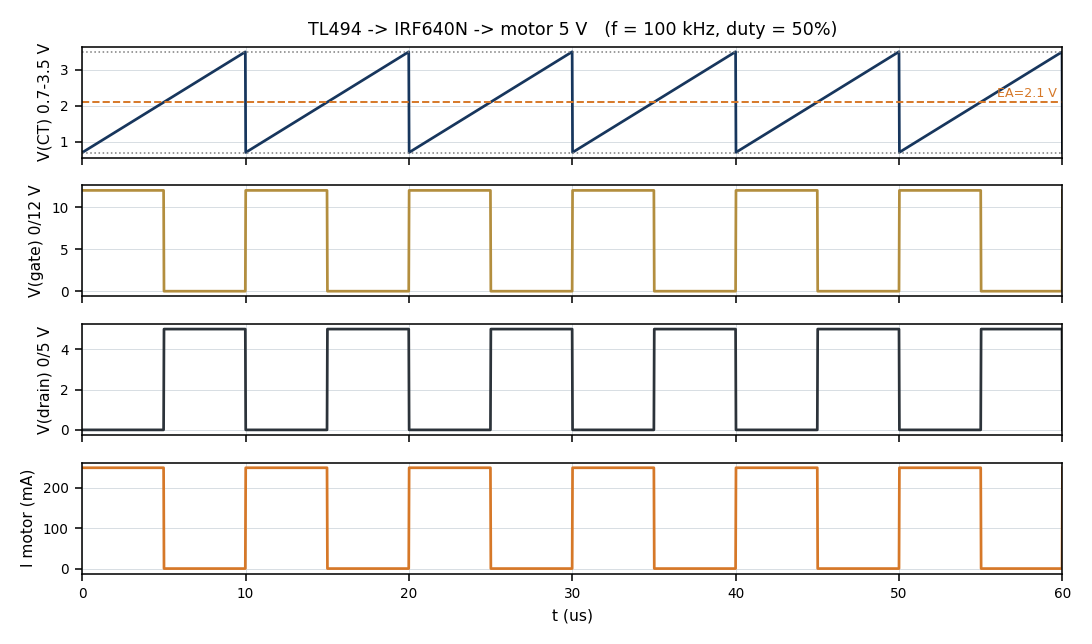
\includegraphics[width=0.72\textwidth]{figs/tl494_pwm_waveforms.png}
  \end{center}
  \begin{itemize}
    \item Sierra $0.7$–$3.5\,\mathrm{V}$ vs $EA=2.1\,\mathrm{V}$ $\Rightarrow$ duty $50\%$.
    \item $V_{GS}$ $0/12\,\mathrm{V}$, $V_{DS}$ invertida $5/0\,\mathrm{V}$,
      corriente media del motor $\approx 198\,\mathrm{mA}$.
  \end{itemize}
\end{frame}

% ---------------------------------------------------------------------
\begin{frame}{Resultados verificados en LTspice XVII}
  \begin{table}
    \small
    \begin{tabular}{lll}
      \toprule
      Magnitud & Medido & Esperado \\
      \midrule
      Periodo del PWM (2 ciclos) & \SI{20}{\micro\second} & $2/f = \SI{20}{\micro\second}$ ($f=100\,\mathrm{kHz}$) \\
      $V_{GS}$ promedio & $6.09\,\mathrm{V}$ & $12\,\mathrm{V}\cdot 0.5 \approx 6\,\mathrm{V}$ ($duty=50\%$) \\
      $V_{GS,on}$ real & $0\leftrightarrow 12\,\mathrm{V}$ & driver $\ge 10\,\mathrm{V}$ (IRF640N) \\
      $EA$ (dinámica) & $2.10\,\mathrm{V}$ & $2.1\,\mathrm{V}$ (divisor REF) \\
      Referencia interna & $5.00\,\mathrm{V}$ & $5\,\mathrm{V}$ \\
      Sierra $C_T$ & $0.707$–$3.49\,\mathrm{V}$ & $0.7$–$3.5\,\mathrm{V}$ \\
      $I_{motor}$ media & $198\,\mathrm{mA}$ & $\approx 250\,\mathrm{mA}\cdot 0.5 +$ pérdidas \\
      \bottomrule
    \end{tabular}
  \end{table}
  \begin{block}{Modelo}
    `tl494\_educativo.sub` es un modelo \textbf{pedagógico por bloques} (no el
    circuito interno de TI): reproduce bloques, no cada transistor del silicio.
  \end{block}
\end{frame}

% ---------------------------------------------------------------------
\begin{frame}{Notas de diseño (motores + PWM)}
  \begin{itemize}
    \item \textbf{Frecuencia:} $>20\,\mathrm{kHz}$ evita zumbido audible y reduce rizado;
      para motores pequeños $50$–$100\,\mathrm{kHz}$ es buen punto.
    \item \textbf{Dead-time:} DTC evita cruce simultáneo en etapa push-pull;
      con salida única se deja arriba (sin límite).
    \item \textbf{Corriente de pico} al arrancar (inrush/bloqueo): medir antes de
      fijar $R_{DS}$ y el bus; en el diseño se usa la envolvente $250/400\,\mathrm{mA}$.
    \item \textbf{Pérdidas:} $P = I^2 R_{DS(on)}$ (con ~$0.15\,\mathrm{\Omega}$: $\le 24\,\mathrm{mW}$)
      + conmutación ($Q_g\cdot f$).
    \item El \textbf{gate} es capacitivo: la corriente de driver fluye solo al
      conmutar ($I_{G,avg} \approx Q_g f$).
  \end{itemize}
\end{frame}

% ---------------------------------------------------------------------
\begin{frame}{Resumen}
  \begin{itemize}
    \item El \textbf{TL494} genera PWM con: oscilador $R_TC_T$ ($f=1.1/R_TC_T$),
      referencia 5 V, EA (realimentación), DTC (límite de ancho) y comparador PWM.
    \item \textbf{Duty} $= \big(\min(EA,DTC)-0.7\big)/2.8$; con $EA=2.1\,\mathrm{V}$:
      $50\%$.
    \item En el diseño: TL494 a $12\,\mathrm{V}$ $\to$ $R_G$ $\to$ \textbf{IRF640N}
      $\to$ motor $5\,\mathrm{V}$; verificado en LTspice: $100\,\mathrm{kHz}$, $50\%$,
      $V_{GS}=0/12\,\mathrm{V}$, $I_{motor}\approx 198\,\mathrm{mA}$.
    \item El modelo educativo (`tl494\_educativo.sub`) es reutilizable para
      estudiar control de duty y dead-time.
  \end{itemize}
\end{frame}

% ---------------------------------------------------------------------
\begin{frame}{Preguntas de verificación}
  \begin{enumerate}
    \item ¿Qué formula la frecuencia del TL494?
      \uncover<2->{\emph{($f = 1.1/(R_TC_T)$; con $11\,\mathrm{k}$ + $1\,\mathrm{nF}$ $\Rightarrow 100\,\mathrm{kHz}$.)}}
    \item ¿Con qué entradas se fija el ciclo de trabajo?
      \uncover<3->{\emph{($\min(EA, DTC)$ comparado con la sierra $0.7$–$3.5\,\mathrm{V}$.)}}
    \item ¿Qué hace el DTC (pin 4)?
      \uncover<4->{\emph{(Limita el ancho máximo / inserta dead-time.)}}
    \item ¿Por qué el driver está en $12\,\mathrm{V}$ y no en $3.3\,\mathrm{V}$?
      \uncover<5->{\emph{(El IRF640N necesita $V_{GS}\ge 10\,\mathrm{V}$.)}}
    \item ¿Qué pasa si el motor se bloquea (400 mA > 250 mA)?
      \uncover<6->{\emph{((250-400 mA) sube $I^2R_{DS}$ y el rizado; hay que asegurar el bus y el derating del MOSFET.)}}
  \end{enumerate}
\end{frame}

\end{document}
